\chapter{基于原型构造的LDPC码}
\section{LDPC码的原型}
每一个LDPC码都对应着一个Tanner图,也可称为原型,或者称为基本图。如下图,
\begin{center}
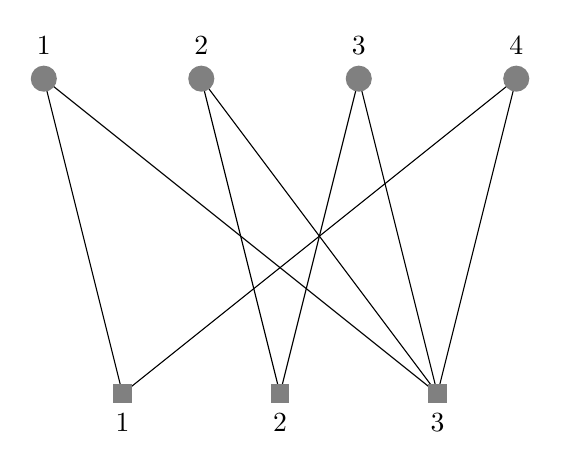
\begin{tikzpicture}
[check/.style={rectangle,fill=black!50,thick},
bit/.style={circle,fill=black!50,thick}]
\draw (-3,4) -- (-2,0);
\draw (3,4) -- (-2,0);
\draw (-1,4) -- (0,0);
\draw (1,4) -- (0,0);
\draw (-3,4) -- (2,0);
\draw (-1,4) -- (2,0);
\draw (1,4) -- (2,0);
\draw (3,4) -- (2,0);
\node[bit] at ( 1,4) [/tikz/label=above:3] {}; 
\node[bit] at (-1,4) [/tikz/label=above:2] {};
\node[bit] at (-3,4) [/tikz/label=above:1] {};
\node[bit] at ( 3,4) [/tikz/label=above:4] {}; 
\node[check] at ( 0,0) [/tikz/label=below:2] {}; 
\node[check] at ( 2,0) [/tikz/label=below:3] {}; 
\node[check] at (-2,0) [/tikz/label=below:1] {};
\end{tikzpicture}
\figurecaption{基本图}
\end{center}
该基本图描述的LDPC码的校验矩阵记为
\begin{equation}
    H_b = \left(
      \begin{array}{cccc}
        1 & 0 & 0 & 1 \\
        0 & 1 & 1 & 0 \\
        1 & 1 & 1 & 1 
      \end{array} \right)
\end{equation}
可以通过叠加基本图构造有结构的LDPC码。
比如,先复制m次基本图,得到簇状的Tanner图,如下图。
\begin{center}
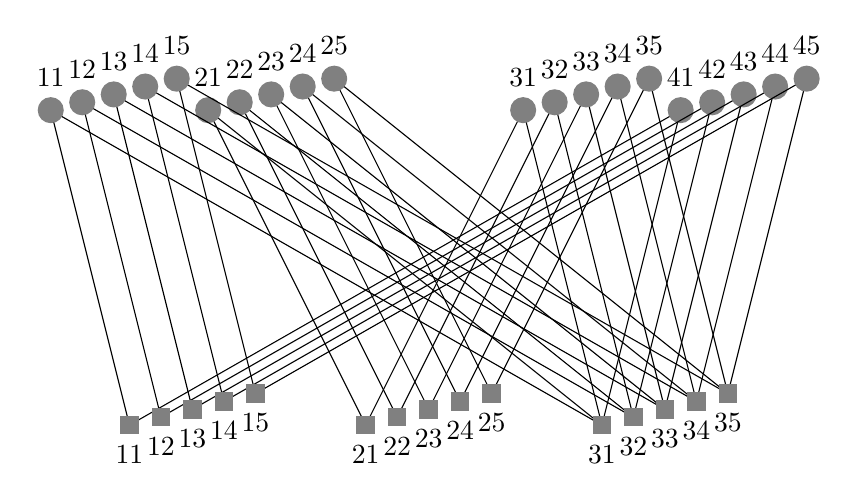
\begin{tikzpicture}
[bit/.style={circle,fill=black!50,thick},
check/.style={rectangle,fill=black!50,thick}]
\foreach \x / \y / \z in {0/1/0,0.4/2/0.1,0.8/3/0.2,1.2/4/0.3,1.6/5/0.4}
{
	\draw[shift={(\x,\z)}] (-4,4) -- (-3,0);
	\draw[shift={(\x,\z)}] (4,4) -- (-3,0);
	\draw[shift={(\x,\z)}] (-2,4) -- (0,0);
	\draw[shift={(\x,\z)}] (2,4) -- (0,0);
	\draw[shift={(\x,\z)}] (-4,4) -- (3,0);
	\draw[shift={(\x,\z)}] (-2,4) -- (3,0);
	\draw[shift={(\x,\z)}] (2,4) -- (3,0);
	\draw[shift={(\x,\z)}] (4,4) -- (3,0);
	\node[bit,shift={(\x,\z)}] at ( 2,4) [/tikz/label=above:3\y] {}; 
	\node[bit,shift={(\x,\z)}] at (-2,4) [/tikz/label=above:2\y] {};
	\node[bit,shift={(\x,\z)}] at (-4,4) [/tikz/label=above:1\y] {};
	\node[bit,shift={(\x,\z)}] at ( 4,4) [/tikz/label=above:4\y] {}; 
	\node[check,shift={(\x,\z)}] at ( 0,0) [/tikz/label=below:2\y] {}; 
	\node[check,shift={(\x,\z)}] at ( 3,0) [/tikz/label=below:3\y] {}; 
	\node[check,shift={(\x,\z)}] at (-3,0) [/tikz/label=below:1\y] {};
}
\end{tikzpicture}
\end{center}
然后将基本图对应的$H_b$中为$1$的元素换为来自置换矩阵集合的元素。即
\begin{equation}
    H = \left(
      \begin{array}{cccc}
        P^2 & 0 & 0 & P^5 \\
        0 & P^5 & P^1 & 0 \\
        P^4 & P^3 & P^2 & P^4 
      \end{array} \right)
\end{equation}
其中$p^i$对应循环置换矩阵,比如
\begin{equation}
    P^2 = \left(
      \begin{array}{ccccc}
        0 & 0 & 0 & 0 & 1 \\
        1 & 0 & 0 & 0 & 0 \\
        0 & 1 & 0 & 0 & 0 \\
        0 & 0 & 1 & 0 & 0 \\
        0 & 0 & 0 & 1 & 0 
      \end{array} \right)
\end{equation}
此时构造出来的LDPC码的Tanner图如下
\begin{center}
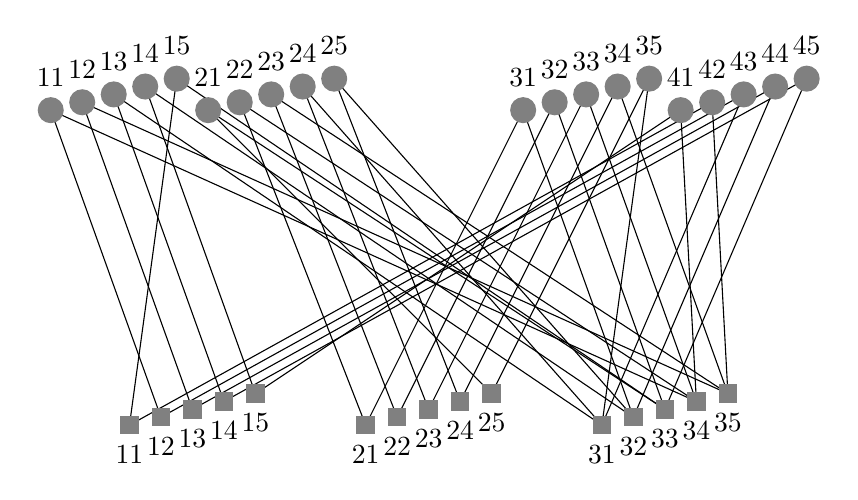
\begin{tikzpicture}
[bit/.style={circle,fill=black!50,thick},
check/.style={rectangle,fill=black!50,thick}]
%p2
	\draw (-2.4,4.4) -- (-3,0);
	\draw (-4,4) -- (-2.6,0.1);
	\draw (-3.6,4.1) -- (-2.2,0.2);
	\draw (-3.2,4.2) -- (-1.8,0.3);
	\draw (-2.8,4.3) -- (-1.4,0.4);
%p5
	\draw (4.4,4.1) -- (-3,0);
	\draw (4.8,4.2) -- (-2.6,0.1);
	\draw (5.2,4.3) -- (-2.2,0.2);
	\draw (5.6,4.4) -- (-1.8,0.3);
	\draw (4,4) -- (-1.4,0.4);
%p5
	\draw (-1.6,4.1) -- (0,0);
	\draw (-1.2,4.2) -- (0.4,0.1);
	\draw (-0.8,4.3) -- (0.8,0.2);
	\draw (-0.4,4.4) -- (1.2,0.3);
	\draw (-2,4) -- (1.6,0.4);
%p4
	\draw (-3.2,4.2) -- (3,0);
	\draw (-2.8,4.3) -- (3.4,0.1);
	\draw (-2.4,4.4) -- (3.8,0.2);
	\draw (-4,4)   -- (4.2,0.3);
	\draw (-3.6,4.1) -- (4.6,0.4);
%p3
	\draw (-0.8,4.3) -- (3,0);
	\draw (-0.4,4.4) -- (3.4,0.1);
	\draw (-2,4)   -- (3.8,0.2);
	\draw (-1.6,4.1) -- (4.2,0.3);
	\draw (-1.2,4.2) -- (4.6,0.4);
%p2
	\draw (3.6,4.4) -- (3,0);
	\draw (2,4)   -- (3.4,0.1);
	\draw (2.4,4.1) -- (3.8,0.2);
	\draw (2.8,4.2) -- (4.2,0.3);
	\draw (3.2,4.3) -- (4.6,0.4);
%p4
	\draw (4.8,4.2) -- (3,0);
	\draw (5.2,4.3) -- (3.4,0.1);
	\draw (5.6,4.4) -- (3.8,0.2);
	\draw (4,4)   -- (4.2,0.3);
	\draw (4.4,4.1) -- (4.6,0.4);
\foreach \x / \y / \z in {0/1/0,0.4/2/0.1,0.8/3/0.2,1.2/4/0.3,1.6/5/0.4}
{
	\draw[shift={(\x,\z)}] (2,4) -- (0,0);
	\node[bit,shift={(\x,\z)}] at ( 2,4) [/tikz/label=above:3\y] {}; 
	\node[bit,shift={(\x,\z)}] at (-2,4) [/tikz/label=above:2\y] {};
	\node[bit,shift={(\x,\z)}] at (-4,4) [/tikz/label=above:1\y] {};
	\node[bit,shift={(\x,\z)}] at ( 4,4) [/tikz/label=above:4\y] {}; 
	\node[check,shift={(\x,\z)}] at ( 0,0) [/tikz/label=below:2\y] {}; 
	\node[check,shift={(\x,\z)}] at ( 3,0) [/tikz/label=below:3\y] {}; 
	\node[check,shift={(\x,\z)}] at (-3,0) [/tikz/label=below:1\y] {};
}
\end{tikzpicture}
\end{center}
\section{LDPC分组码的构造}
设计码率为$R=b/c$的LDPC分组码的原型是一个二分图,有$c$个变量节点和$c-b$个校验节点。
它能生成不同码长的,设计码率为$R$,有相同的度分布的分组码。
GF($q$)为含$q=2^m$个元素的有限域,其中$m$为在GF($q$)代表一个符号所需的位数。令$M$为原型叠加数。通过以下两步从原型的$(c-b)\times c$邻接矩阵$\mathbf{B}=[B_{i,j}]$构造码长为$n_{BC}=Mc$的$q$元LDPC分组码:
\begin{enumerate}
\item 将$\mathbf{B}$中的非零元$B_{i,j}$替换为随机选择的$M \times M$置换矩阵,将$\mathbf{B}$中的零元$B_{i,j}$替换为$M \times M$零矩阵。此时得到对应于$\mathbf{B}$的二元校验矩阵$\mathbf{H}$;
\item 将$\mathbf{H}$中非零元替换为从有限域GF($q$)中随机选取的元素,得到LDPC分组码的$q$元校验矩阵$\mathbf{H}_{BC}$。
\end{enumerate}
对于LDPC分组码,必须等待整个码块接受完毕才能执行置信传播解码算法。故$q$元LDPC分组码的解码延时为
\[
T_{BC}=n_{BC}\cdot m = Mmc
\]
\section{LDPC卷积码的构造}
LDPC卷积码也可以通过叠加原型来构造。
原型的基本矩阵为$(c-b)\times c$的$\mathbf{B}$,以此构造码率为$R=b/c$的LDPC卷积码。首先构造$\mathbf{B}_{SC}$
\begin{equation}
    \mathbf{B}_{SC} = \left[
          \begin{array}{ccc}
            \mathbf{B}_0& & \\
            \mathbf{B}_1 & \mathbf{B}_0 & \\
            \vdots & \mathbf{B}_1 & \ddots \\
            \mathbf{B}_{m_s} & \vdots & \ddots \\
             & \mathbf{B}_{m_s} & \ddots \\
             & & \ddots 
          \end{array} \right]
\end{equation}
其中$m_s$为记忆因子,即当前原型与前一个原型相连的边数。$\mathbf{B}_0 , \mathbf{B}_1 , \dots , \mathbf{B}_{m_s}$为$(c-b)\times c$矩阵,且满足
\[
\sum^{m_s}_{i=0} \mathbf{B}_i = \mathbf{B}
\]
然后将$\mathbf{B}_{SC}$中的非零元替换为随机选择的$M \times M$置换矩阵,将$\mathbf{B}_{SC}$中的零元替换为$M \times M$零矩阵,得到LDPC卷积码校验矩阵$\mathbf{H}_{SC}$。
最后将$\mathbf{H}_{SC}$中的非零元替换为从有限域GF($q$)中随机选取的元素,得到LDPC卷积码的$q$元校验矩阵$\mathbf{H}_{BC}$,其限制长度(决定了非零对角带的最大宽度),为$v_s=(m_s+1)Mc$。

本文为简单起见,采用$m_s=1$,并且只考虑正则$(d_v,d_c)$LDPC卷积码,即$\mathbf{H}_{SC}$中每行重量为$d_c$,每列重量为$d_v$。
同时限定随机选择置换矩阵的方法如下。
选择两个$(c-b)\times c$矩阵$\mathbf{B}_0$和$\mathbf{B}_1$,使得$\mathbf{B}_0 + \mathbf{B}_1$为正则$(d_v,d_c)$矩阵。LDPC分组码的基本矩阵为
\begin{equation}
    \mathbf{B}_{BC} = \left[
          \begin{array}{cc}
            \mathbf{B}_0 & \mathbf{B}_1\\
            \mathbf{B}_1 & \mathbf{B}_0
          \end{array} \right]_{2(c-b)\times 2c}
\end{equation}
然后使用第二节的原型叠加方法构造LDPC分组码的校验矩阵
\begin{equation}
    \mathbf{H}_{BC} = \left[
          \begin{array}{cc}
            \mathbf{H}_0 & \mathbf{H}_1\\
            \mathbf{H}_1 & \mathbf{H}_0
          \end{array} \right]_{2(c-b)M \times 2cM}
\end{equation}
对于LDPC卷积码,使用相同的$\mathbf{B}_0$和$\mathbf{B}_1$,得到正则$(d_v,d_c)$LDPC卷积码的基本矩阵为
\begin{equation}
    \mathbf{B}_{SC} = \left[
          \begin{array}{ccccc}
            \mathbf{B}_0 & & & & \\
            \mathbf{B}_1 & \mathbf{B}_0 & & & \\
             & \mathbf{B}_1 & \mathbf{B}_0 & & \\
             & & \mathbf{B}_1 & \mathbf{B}_0 & \\
             & & & \mathbf{B}_1 & \ddots \\
             & & & & \ddots
          \end{array} \right]
\end{equation}
然后使用原型叠加方法构造LDPC卷积码的校验矩阵
\begin{equation}
    \mathbf{H}_{SC} = \left[
          \begin{array}{ccccc}
            \mathbf{H}_0 & & & & \\
            \mathbf{H}_1 & \mathbf{H}_0 & & & \\
             & \mathbf{H}_1 & \mathbf{H}_0 & & \\
             & & \mathbf{H}_1 & \mathbf{H}_0 & \\
             & & & \mathbf{H}_1 & \ddots \\
             & & & & \ddots
          \end{array} \right]
\end{equation}
基于以上构造规则,可以使用其他的基本矩阵(见下表)构造LDPC分组码校验矩阵$\mathbf{H}_{BC}$与LDPC卷积码校验矩阵$\mathbf{H}_{SC}$。当原型叠加数为$M$,有限域元素个数为$q=2^m$时,LDPC分组码的码长和LDPC卷积码的限制长度都等于$2Mmc$。
\begin{center}
\tablecaption{构造LDPC分组码和LDPC卷积码的组成矩阵}
\begin{tabular}{c|c|c}
 \hline
码 & 组成矩阵 &码长/限制长度 \\ \hline
(2,4)-正则 & 
$\mathbf{B}_0 = \mathbf{B}_1 = [\begin{array}{cc} 1&1 \end{array}]$ & 4Mm \\ \hline
(3,6)-正则 & 
 $\mathbf{B}_0 = [\begin{array}{cc} 2&1 \end{array}]$,$\mathbf{B}_1 = [\begin{array}{cc} 1&2 \end{array}]$ & 4Mm \\ \hline
(3,9)-正则 & 
 $\mathbf{B}_0 = [\begin{array}{ccc} 1&2&2 \end{array}]$,$\mathbf{B}_1 = [\begin{array}{ccc} 2&2&1 \end{array}]$ & 6Mm \\ \hline
(3,12)-正则 & 
 $\mathbf{B}_0 = [\begin{array}{cccc} 1&1&2&2 \end{array}]$,$\mathbf{B}_1 = [\begin{array}{cccc} 2&2&1&1 \end{array}]$ & 8Mm \\ \hline

\end{tabular}
\end{center}